\chapter{Results and Analysis}
%%This is the chapter in which you review the outcomes, and
%%critique the outcomes process.  You may include user evaluation here
%%too.

\section{Introduction}
Throughout this chapter we look at the results of our quantitative study, and analyse them to determine the answers to the questions laid out in section \ref{overallgoals}, as well as how well the system meets our requirements, and ultimately our goals. 

\section{Overview}
For each of the systems involved in the study, we evaluted a the time taken to complete each task, in order to determine the answer to the 5 criteria set out in section \ref{quantitativestudy}.
We also recorded the number of times a user deviated from the expected route, in order to gauge efficiency, though this was a less important measurement.
These heuristics allowed us to test for speed, as well as give us a more quantitative description of how clear and simple the system may be to use.

It is worth noting that, through the study, the participants were not aware that they would be timed to complete the task.
We hoped that by not alerting them of this fact, we would maintain realistic use of the system, and that users would not attempt to complete tasks quickly.
This is important as we are calculating speed, so we want it to be accurate, and if the user is rushing or attempting to complete the tasks quickly, they have the potential to affect the outcome both, either by completing it quicker than usual, or by making mistakes resulting from rushing.
Ultimately we decided to try and ensure this doesn't happen.

\section{Heuristics}

\subsection{Speed - Time Taken to Store} \label{storespeed}
Within the regular file system, when storing a snippet, the users would need to create a blank text file to store the snippet. This was quick, but meant there was no standardisation of storage, and different files may contain different data, or none at all. 
However, this did mean that storing the snippet was much quicker, as simply creating the file and pasting the snippet in to it was fast.

As for Gist, there were more steps between creating the snippet and saving it, though this did then incorporate meta data and a standardised method of storage. 
Equally the time period of creating the snippet to saving the snippet was only a few second (5 to 10) longer than that of the text files.

Finally, Shnip It had the longest time to create and save the snippets, due to the inclusion of even more metadata, however again this was around 5 to 10 seconds longer than Gist.

Speed, however, is two-fold, as we must look at both storage and retrieval. 
Storing the snippet is a one-time execution, and reusing the snippet is a much more common action.
As such, we place more weight on the results of our speed test for snippet retrieval.

\subsection{Speed - Time Taken to Retrieve} \label{speedretrieve}
The regular file system suffered from a number of drawbacks that hampered its speed of retrieval, relating mostly to ambiguity.

Initially, the snippets can be stored altogether, or grouped into folders.
If stored together, the user has only the name of the text file to decide what's in the file and if it's the desired snippet.
It is also very difficult to navigate or search due to the lack of structure.
If a system of folders is introduced, as some users decided to do, further ambiguity can present itself if the structure is not well defined.
It was found that users would forget which folder the snippet they required was in, and would spend periods of time navigating in and out of folders. 
This also does not solve the problem of only having the file name to discern what the snippet was.

With Gist, the metadata was useful, and the standardised storage method allows a better representation of the snippets than the file storage system. 
A portion of the code is also displayed when the snippets are listed, allowing the user to see the first few lines of the code, and aid in discerning if this is the correct snippet.
Despite this, users were found to spend a good portion of time scrolling up and down through the list of snippets in order to find the one they required, due to the nature of the user interface and minimal metadata. 
The Gists did not always have descriptions, as some users did not provide them, and there were no tags to quickly digest what the snippet contained.

Finally, Shnip It had the fastest retrieval time, though beating Gist on average by 2 seconds per snippet, but bettering the regular file system by over a minute.
It was seen that users would more accurately select the correct snippet first time due to the extra metadata provided, and the clearer layout of listing the snippets.
However, when the user did pick the incorrect snippet, the website had to load the snippet for them to discover it was incorrect, and as such they would have to go back to the listing of snippets, causing two page loads.
This could be mitigated by providing a method of viewing the code without clicking on it, such as Gist does, but to present it on mouseover rather than embedded in the search results, as to refrain from cluttering the page.

\subsection{Speed - Overall Results}
Throughout the speed test, it was seen that the system with the least detail was faster to store snippets in, but that this 'cutting corners' led to a much increased time to retrieve those snippets. 
As retrieval occurs more frequently than storing, this played a large factor in our judgement of overall speed.
As such, we feel this satisfies the requirement of our system to be on par with existing systems.

We leave for a future study the effects of these systems with a small amount of snippets versus the same systems filled with a large amount of snippets, and test retrieval times in those situations.
Our hypothesis for such a study is that the negative effect of high load on Shnip It and Gist will be minimal, but that same effect will be far greater on the regular file system, further promoting Shnip It.

%% TODO Should we do something about testing an empty or low amount of snippets versus a high amount of snippets?

\subsection{Deviations - Efficiency}
Before discussing deviations, it is worth repeating that this heuristic is not as important to use, as it is not a goal of our system to be efficient - that is, to minimise the path from start to end - and so is analysed in less detail.
It was, however, data available to us, and as such is looked in to as some measurement.
We will not, however, be performing a deeper analysis on efficiency.

We considered a deviation to be any scenario where an action was taken that led to some unnecessary intermediary page or folder, such as when searching for a specific call-to-action on a website, or entering a folder which doesn't hold the contents you're looking for.
As such, the optimum route is one where no deviations occur, and all pages viewed are necessary to achieve the goal.

For some tasks, a short cut would result in a more optimum route (such as a notification leading straight to a specific page with a single button press). In these cases, it was chosen to ignore shortcuts for the purpose of this analysis, and to treat them as equal to the optimum route if the user made use of them.

It was found that storing a snippet in the regular file system often resulted in several deviations, as users would navigate between folders, exploring the current contents before deciding where to store the snippet.
On the contrary, very little, if any, deviation was found when using Gist or Shnip It, which suggests a simple and clear system with little ambiguity.

As for snippet retrieval, there was great deviation found in the regular file system, most likely due to having just the filename to distinguish the files. 

Gist had very little deviation, due in part to its metadata, but also because part of the snippet is visible within the snippet list.
Once the snippet was present on the page, there was almost no deviation before it was found.

Shnip It was slightly outperformed in this case, as similar snippets can be mistaken for each other, and no part of the code is given until the snippet is opened.
The suggestion provided in section \ref{speedretrieve} of showing the snippet on mouse rollover would mitigate this extra deviation, and in most cases eliminate it entirely.

As such, we can again say Shnip It is on par with existing solutions, within our margins, and that it can be further improved, both in speed and efficiency, with the suggestion mentioned.

\subsection{Limitations of our Analysis}
Our analysis is subject to some limitations, by nature of the task, and constraints out of our control.

Users were instructed to create their own folder structure for the task, and as such the exact structures differed, though they were verbally advised to group the snippets by coding language and then functionality. 
This meant that some users had deeper folder structures than others, while some had no organisation at all. 
As such, speed was somewhat affected in these edge cases, though the majority of users (9) had a maximum folder depth of 2, as recommended. 1 user had no folder structure, 1 had a depth of 1 and the last had a maximum depth of 3.

Furthermore, deviations for the file system were then regarded as those folders entered and exited unnecessarily, in hindsight, and also files opened that weren't required.
These figures evened out amongst the different file structures, and so didn't affect deviations as much.
Speed, however, appeared to be reduced by the lack of structure, though this is impossible for us to prove from our results due to the nature of the data collected, so we just note it as a limitation.

We performed no analysis of participants skill level with either the file system or with Gist prior to the study, and as such we don't analyse the results as first time users for these systems. 
Instead, they're analysed as that of 'at least a beginner user'.
We also examine the use of Shnip It as 'at most that of a beginner', and so we use this crossover level of beginner through our analysis of the results.

\section{Analysis Breakdown}
\subsection{Overview}
We now look deeper at our results, with our original goals in mind.\\
As a reminder for the reader, these are:

\textbf{Goal 1: To create a snippet repository that is at least on par with existing solutions for storage and retrieval of snippets}. \\
\textbf{Goal 2: To create a system that enables users to collaborate on their saved snippets, to promote quality and keep them up to date}.

We use the quantitative elements of this study to assess the first goal, being the 6 tasks and the timed screen recording, as this provides us with the necessary numerical analysis.
We look further into the second goal in the next chapter, as we evaluate the post-study questionnaires to examine more qualitative data regarding the users preferred systems and their thoughts and opinions surrounding the collaborative elements.

For ease of reading, throughout this analysis we refer to the default file system as \textbf{FS}, Gist as \textbf{Gist}, and Shnip It as \textbf{SI}.

\subsection{Analysis of Speed}
Firstly, we present a clustered column graph in figure \ref{speedresultsgraph} detailing the breakdown of speed across the 3 systems, detailing the users average speeds in the 6 tasks.

\begin{sidewaysfigure}[htbp]
\centering
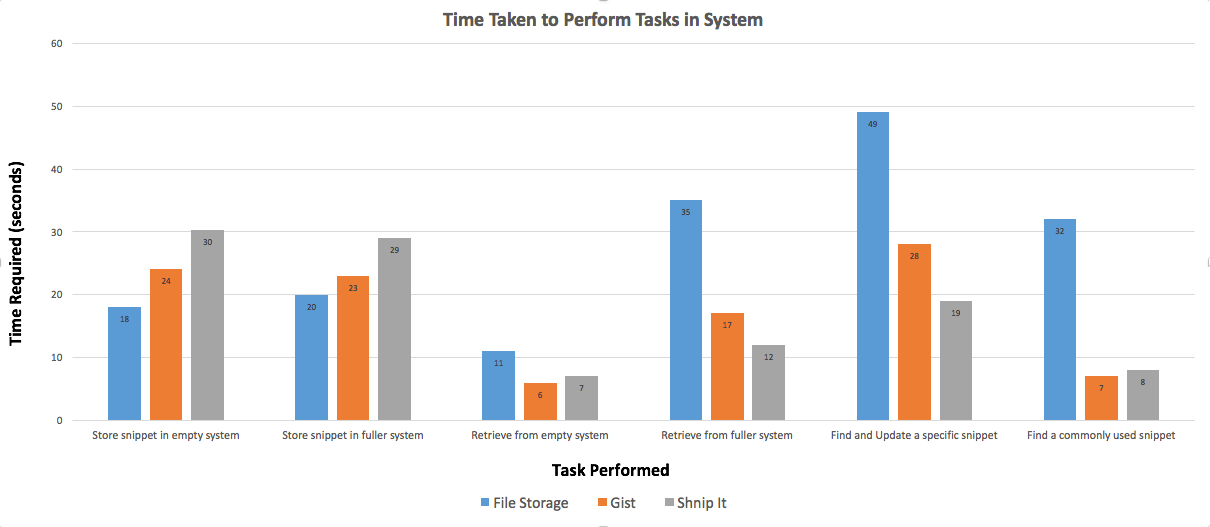
\includegraphics[width=20cm]{SpeedResultsGraph}
\caption{Time taken in seconds per task performed, for each of the 3 systems \label{speedresultsgraph}}
\end{sidewaysfigure}

This graph details the time, in seconds, it takes a user to complete a task, and is measured from the moment the user first interacts with the system, to the moment the final keypress or action button is clicked. 
For retrieval, this includes highlighting and copying the snippet, and for storage this is the action which saves the snippet.
Smaller bars represent a faster system, and as such, the more desireable outcome.

It is interesting to note that, for storage, FS consistently achieved the fastest time, however in all other tasks it was deemed the slowest, and in some cases, by a considerable margin. 
The opposite was true for Gist, scoring slower in storage, but faster in retrieval.
It's clear SI was the slowest in retrieval, and this seemed mostly due to the extra metadata that users had to input, though this then went on to ensure it was much faster than FS for retrieval, and in good competition with Gist, being the fastest for 2 of the 4 retrieval tests, and only a second slower otherwise, on average.

As noted in section \ref{storespeed}, more importance was placed on retrieval, as it's a more common action than storage.
As such, this graph provides a positive outlook on our first goal: that the system is at least on par with current solutions. 

We now look further in-depth into the statistical analysis of our individual tasks, and then go on to provide some insight on observed behaviours gleaned from the screen recordings in section \ref{observationanalysis}.

\subsection{Analysis of Speed by Task}
\subsubsection{Task 1: Storing Snippet within an Empty System}
\begin{table}[H]
\label{speedtabletask1}
\begin{tabular}{ll}
\hline
\textbf{System} & \textbf{Speed (s.d. err)} \\ \hline
FS              & 18 (0.2462)     \\ 
Gist            & 24 (0.4082)     \\ 
SI              & 30 (0.5383)     \\ \hline
\end{tabular}
\end{table}

Mean speed differed statistically significantly between systems. \\
(F = 217.7033, p \textless 0.0001)

Gist speed significantly faster than SI (p \textless 0.001). \\
FS speed significantly faster than SI (p \textless 0.001). \\
FS speed significantly faster than Gist (p \textless 0.001). \\

Not in line with Goal 1 of the system, though this test for storage is less important than retrieval.

\subsubsection{Task 2: Storing Snippet within a Fuller System}
\begin{table}[H]
\label{speedtabletask2}
\begin{tabular}{ll}
\hline
\textbf{System} & \textbf{Speed (s.d. err)} \\ \hline
FS              & 20 (0.2132)     \\ 
Gist            & 23 (0.3257)     \\ 
SI              & 29 (0.2752)     \\ \hline
\end{tabular}
\end{table}

Mean speed differed statistically significantly between systems. \\
(F = 277.2, p \textless 0.0001)

Gist speed significantly faster than SI (p \textless 0.001). \\
FS speed significantly faster than SI (p \textless 0.001). \\
FS speed significantly faster than Gist (p \textless 0.001). \\

Again, not in line with Goal 1 of the system, however, again, this test for storage is less important than retrieval.

\subsubsection{Task 3: Retrieving Snippet from within an Empty System}
\begin{table}[H]
\label{speedtabletask3}
\begin{tabular}{ll}
\hline
\textbf{System} & \textbf{Speed (s.d. err)} \\ \hline
FS              & 11 (0.3128)     \\ 
Gist            & 6 (0.2132)     \\ 
SI              & 7 (0.2843)     \\ \hline
\end{tabular}
\end{table}

Mean speed differed statistically significantly between systems. \\
(F = 102.161, p \textless 0.0001)

Gist speed significantly faster than FS (p \textless 0.001). \\
SI speed significantly faster than FS (p \textless 0.001). \\
Analysis did not show a significant value for SI vs Gist (p = 0.07396). \\

For retrieval in an empty system, Goal 1 is met, as there is no significant difference between Gist and SI, however both systems are significantly faster than FS.

\subsubsection{Task 4: Retrieving Snippet from within a Fuller System}
\begin{table}[H]
\label{speedtabletask4}
\begin{tabular}{ll}
\hline
\textbf{System} & \textbf{Speed (s.d. err)} \\ \hline
FS              & 35 (0.4606)     \\ 
Gist            & 17 (0.5198)     \\ 
SI              & 12 (0.2462)     \\ \hline
\end{tabular}
\end{table}

Mean speed differed statistically significantly between systems. \\
(F = 804.637, p \textless 0.0001)

Gist speed significantly faster than FS (p \textless  0.001). \\
SI speed significantly faster than FS (p \textless  0.001). \\
SI speed significantly faster than Gist (p \textless  0.001). \\

For retrieval in a fuller system, Goal 1 is exceeded, as SI is significantly faster than both other systems.


\subsubsection{Task 5: Finding and Updating a Specific Snippet}
\begin{table}[H]
\label{speedtabletask5}
\begin{tabular}{ll}
\hline
\textbf{System} & \textbf{Speed (s.d. err)} \\ \hline
FS              & 49 (1.3842)     \\ 
Gist            & 28 (0.3693)     \\ 
SI              & 19 (0.4167)     \\ \hline
\end{tabular}
\end{table}

Mean speed differed statistically significantly between systems. \\
(F = 321.72972, p \textless 0.0001)

Gist speed significantly faster than FS (p \textless  0.001). \\
SI speed significantly faster than FS (p \textless  0.001). \\
SI speed significantly faster than Gist (p \textless  0.001). \\

Again, Goal 1 has been exceeded, with SI being significantly faster than both other systems. 
It is interesting to note the large deviation in speeds shown by users of FS, and may relate to the folder structure chosen by the participants, or simply that they struggled to find the specified snippet due to the lack of search functions in FS.

\subsubsection{Task 6: Finding a Commonly Used Snippet}
\begin{table}[H]
\label{speedtabletask6}
\begin{tabular}{ll}
\hline
\textbf{System} & \textbf{Speed (s.d. err)} \\ \hline
FS              & 32 (0.8539)     \\ 
Gist            & 7 (0.1930)     \\ 
SI              & 8 (0.3015)     \\ \hline
\end{tabular}
\end{table}

Mean speed differed statistically significantly between systems. \\
(F = 689.31443, p \textless 0.0001)

Gist speed significantly faster than FS (p \textless  0.001). \\
SI speed significantly faster than FS (p \textless  0.001). \\
Analysis did not show a significant value for SI vs Gist (p = .0168). \\

For this final test of finding a commonly used snippet, Goal 1 is met, as there is no significant difference between Gist and SI, and both systems are significantly faster than FS.
The reason here is that finding a commonly used snippet is mostly identical between the systems, as SI was inspired by Gist, and both utilise a method of specifying a 'starred' snippet for quick retrieval later.


\subsection{Observation of Speed by Task}
Throughout the tasks, number of observations were made regarding the choices the participants made and how the tasks were completed. 
We present them here for consideration in a more qualitative manner.

\subsubsection{Task 1: Storing Snippet within an Empty System}
This task involves using each system in its empty state, with no prior snippets, and simply storing a snippet of code, optionally with metadata.

It was seen that when participants were given a blank folder and a single snippet, they opted not to create any category folders in which to store the snippet, instead opting to simply drop it into the empty folder. 
This meant that FS was quicker than the other two systems, though users seemed to deliberate on how to to store the snippet in the text file, and what metadata to store with it.

Users that utilised the FS as the third system seemed to store more metadata alongside the snippet. 
This may be because they understood what may be useful to store with it, or because they believed it was information the researchers wanted them to store, albeit without being told that.
As such, those users spent longer on the FS than users who utilised it as their first system, where we saw very simple files with minimal information, stored in minimal structure (although this extra time amounted to just a couple of seconds on average).

\subsubsection{Task 2: Storing Snippet within a Fuller System}
This task is mostly similar to the previous one, and similar observations were made.
The speed of task completion is also similar, with slight, single second variances, most likely random and insignifcant in comparison with the previous task.

An interesting observation, however, was that users did spent more time on FS than in the previous task, as now they had to navigate their folder structure, whereas previously, having an empty folder, they would simply create and save a text file.
The extra 2 seconds on average for FS were most likely choosing the folder corresponding to the language of the snippet they were now saving in this system.

\subsubsection{Task 3: Retrieving Snippet from within an Empty System}
In this task, a single snippet was placed within the system, and the users were given information about it and told to retrieve it.
It was the only snippet available within the system, so there was no deliberation over multiple snippets.

Interestingly, despite the users knowing the contents of the system, some users navigated to the wrong folders within the structure, though quickly backed out upon finding no snippet in the folder.
As such, the average time for FS was higher than Gist or SI.

With Gist and SI, the only snippet is immediately available to click on, on the homepage, due to the nature of the systems, and as such allowed users to immediately click it and copy the contents.
This meant they performed faster than FS, though there was no significant difference between the two. 

All users clicked straight through to the snippet, though some took a second or two longer to consider the navigation bar, before realising the snippet was immediately available.

\subsubsection{Task 4: Retrieving Snippet from within a Fuller System}
Within this task is where FS started to struggle, showing its limitations.
Users often clicked through multiple folders, and opened several snippets, before finally finding the snippet they were looking for.
As such the speed of FS greatly drops in this task, and the more complex systems of Gist and SI begin to show their worth.

With Gist and SI, the metadata seemed to play a significant role in expediting the search process for the snippet, allowing users to pinpoint the correct snippet without having to view the contents, or see the actual source code.
This cut down on search time considerably, allowing SI to out perform FS, and even managed to out perform Gist.
It was seen the most likely reason for this is that Gist displays some of the source code along with the snippet, and users seemed to be reading this and taking in more information than with SI, and so slowed down their traversal of the search results.

\subsubsection{Task 5: Finding and Updating a Specific Snippet}
This task began similarly to the previous one, allowing us to again watch users as they retrieved a snippet from a fuller system, though had the added benefit of actioning on a snippet after finding it.

This task had the most variance in time, specifically for FS, as users again struggled to identify the location of the snippet within the folder hierarchy.

Users of Gist and SI found the snippet with much less trouble, making use of the search features and the metadata to find it switfly. 

Editing of the snippet in all systems was relatively simple and understood by all users, with nothing noteworthy to mention.

\subsubsection{Task 6: Finding a Commonly Used Snippet}
At the end of Task 3, users were told to make a mental note of the snippet they added to the system, or to use some functionality of the system they were on, with the knowledge that they would need to navigate back to it many times throughout the test. 
Of course the user did not visit it again until this final task, but it allowed us to instil the the mentality of a commonly used snippet in the user's mind.

Most users used the favourite button on both Gist and SI to save the snippet to a particular location, whereas when using FS, they could only attempt to memorise the location.
As such, FS had a much slower relocation time than Gist and SI, as with the latter, participants could instantly pull up a list containing the snippet. 

One user of SI didn't make use of the favourite button, and instead just searched for the snippet, as in Task 4, which reduced the overall average time by 1 second.
It is unclear whether the user wasn't aware of the favourite function or chose not to use it, however all other 11 participants used the function. 
Further analysis could be done in this area to conclude the reasoning behind this.

\section{Analysis Overview}
This analysis has shown that the first goal of the system has been met: that the system is at least on par with other available systems.
The second goal of the system - that the system enables users to collaborate, ultimately promoting code quality - is yet to be assessed, and will be evaluated via the post-study questionnaire.

\section{Conclusion}
In this chapter we have detailed the results of the quantitative study, as well as perform analysis on them to determine if the first goal of our system has been met.

The next chapter analyses the post-study questionnaire to determine the fate of the second goal, as well as disclose our conclusion on the dissertation and project as a whole.
We also go on to discuss future work available to the system.

 


